\section{Arsitektur Sistem}
Server dibangun dengan arsitektur \emph{RESTful} yang terdiri dari paket \emph{controller}, pemrosesan bahasa alami, pemrosesan ontologi, model serta helper. Paket \emph{controller} berisi kelas Main yang berfungsi sebagai \emph{endpoint} yang akan menerima request dari klien berupa kalimat tanya. Tahapan proses pencarian informasi dilakukan melalui kelas Main hingga membentuk respon berupa objek JSON. Arsitektur sistem yang akan dikembangkan diperlihatkan dalam Gambar \ref{fig:arsitektur_sistem}.

\begin{figure}[ht]
    \centering
    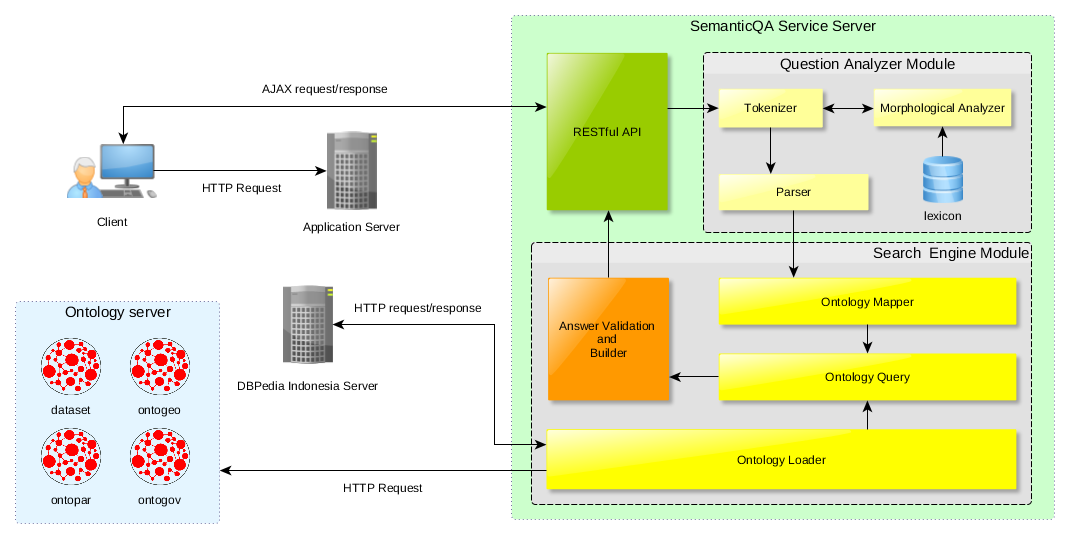
\includegraphics[width=1\textwidth]{bab_4/arsitektur_sistem_revisi_pra_tesis}
    \caption{Arsitektur sistem yang akan dikembangkan}
    \label{fig:arsitektur_sistem}
\end{figure}

Paket pemrosesan bahasa alami terdiri dari kelas Tokenizer, MorphologicalAnalyzer dan Parser. Tokenizer berfungsi untuk mentransformasikan kalimat tanya ke dalam bentuk token-token penyusun kalimat tanya. Tokenizer akan mengembalikan objek model SemanticToken yang terdiri atas \emph{field} kata, kelas kata, fungsi kata di dalam ontologi, representasi alamat URI serta daftar \emph{OWLAxiom} kata yang bersangkutan. \emph{Field} model SemanticToken akan diisi sesuai dengan tahapan-tahapan proses yang dilalui. Pada tahapan tokenisasi, objek model SemanticToken akan diisi dengan kata dan tipe kata sedangkan pada tahapan pemetaan ke dalam ontologi, apabila representasi kata ditemukan di dalam ontologi, maka \emph{field} tipe kata di dalam ontologi, alamat URI serta daftar \emph{OWLAxiom}.

Setelah proses tokenisasi selesai, selanjutnya dilakukan proses pembentukan pohon urai pada kelas Parser. Pohon urai akan memberikan informasi mengenai tipe frasa, fungsi sintaksis frasa serta daftar konstituen pembentuk frasa. Parser akan menerima masukan berupa daftar model SemanticToken yang dibentuk pada proses tokenisasi. Parser akan menghasilkan objek model Sentence yang terdiri dari \emph{field} daftar konstituen yaitu kumpulan objek SemanticToken pembentuk frasa, fungsi sintaksis kata atau frasa serta tipe frasa yang terbentuk.

Objek model Sentence yang dihasilkan oleh Parser selanjutnya akan dikirim ke OntologyMapper untuk memetakan konstituen-konstituen kalimat ke dalam ontologi. Konstituen kalimat dapat berubah bentuk apabila objek ontologi merupakan gabungan dari beberapa konstituen sekaligus, misalnya konstituen frasa nominal terdiri dari [``kabupaten'',``lombok'',``timur''], apabila objek ontologi berupa ``kabupaten\_lombok\_timur'', maka konstituen frasa nominal akan berubah menjadi [``kabupaten\_lombok\_timur''].

Objek model Sentence yang telah melalui proses pemetaan akan dikirimkan ke OntologyQuery untuk membentuk query SPARQL-DL berdasarkan fungsi sintaksis serta representasi konstituen kalimat di dalam ontologi. OntologyQuery juga akan melakukan query serta \emph{reasoning} terhadap ontologi-ontologi yang dibangun dan akan mengembalikan hasil query berupa objek QueryResultModel kepada kelas Main untuk selanjutnya dikirimkan kepada kelas AnswerBuilder. AnswerBuilder selanjutnya akan menganalisa isi dari objek QueryResultModel untuk membentuk kalimat rangkuman jawaban serta mentrasformasikan data-data dari objek QueryResultModel menjadi objek JSON yang kemudian dikirimkan kepada klien.

Adapun langkah pembentukan objek JSON yaitu pertama-tama dilakukan proses pengambilan semua objek hasil \emph{query} SPARQL-DL. Objek hasil \emph{query} berupa URI kemudian dilakukan normalisasi untuk membuang nama domain serta mengganti tanda ``\_'' menjadi tanda spasi sehingga didapatkan bentuk kata yang baik. Selanjutnya proses yang sama juga dilakukan pada objek hasil \emph{query} SPARQL yaitu proses normalisasi bentuk kata. Namun untuk data hasil \emph{query} SPARQL data yang dihasilkan tidak dibentuk menjadi kalimat namun untuk setiap properti dan nilainya dijadikan pasangan \emph{key-value} objek JSON. daftar \emph{key-value} ini nantinya digunakan sebagai isi tabel pada sisi \emph{client}.